\documentclass[manuscript=article]{achemso}

\usepackage[T1]{fontenc}
\usepackage{amsmath}
\usepackage{graphicx}
\usepackage{booktabs}
\usepackage{array}
\usepackage{url}

\SectionNumbersOn
\setkeys{acs}{email=false}

\title{Certified, FCI-Free MPS Response for Analytic State-Averaged DMRG-CASSCF Gradients and Nonadiabatic Couplings}

\author{Yuli Li}
\affiliation[Harvard University]
{Department of Chemistry and Chemical Biology, Harvard University, Cambridge,
Massachusetts 02138, United States}

\abbreviations{CASSCF,SA-CASSCF,DMRG,MPS,FCI,NAC,SHARC}
\keywords{DMRG-CASSCF, analytic gradients, nonadiabatic couplings, PySCF, SHARC}

\newcommand{\Eh}{E_{\mathrm{h}}}
\newcommand{\bfR}{\mathbf{R}}
\newcolumntype{P}[1]{>{\raggedright\arraybackslash}p{#1}}

\begin{document}

\begin{abstract}
Analytic nuclear gradients and nonadiabatic coupling vectors are central
ingredients for locating conical intersections and for propagating
nonadiabatic dynamics with multireference electronic-structure methods.
Complete-active-space self-consistent-field (CASSCF) theory provides a
robust reference near electronic degeneracies, but full configuration
interaction (FCI) in the active space limits the accessible number of active
orbitals.  We present a certified, FCI-free route to state-averaged
DMRG-CASSCF analytic gradients and nonadiabatic couplings built on PySCF and
pyblock2.  The active-space response is carried by matrix product states, so
no dense FCI response vector is ever formed; correctness is established by
finite differences of the solver's own SA-DMRG-CASSCF energies for gradients
and of the SA-DMRG-CASSCF wavefunction for derivative couplings, the latter
through an MPS-native cross-geometry overlap that requires no determinant
expansion.  Each accepted response solution carries an a posteriori
certificate: the true residual of the projected coupled-perturbed equation
and the leakage of the active-space response out of the reference-root space.
On HeH$^+$ CAS(2,2) the MPS-native derivative-coupling finite difference
reproduces the determinant-level reference to $1.6\times10^{-8}$.  The same
machinery is applied to an all-trans polyene $\pi$-space stair reaching
CAS(20,20), whose $3.41\times10^{10}$-determinant active space lies beyond
the reach of FCI-based derivatives; the largest case for which an FCI
reference remains tractable, anthracene CAS(14,14), is used to score the
derivatives directly.  Per-call wall time and peak memory are reported for
the response stages.  A SHARC-compatible interface emits the Hamiltonian,
dipole, gradient, derivative-coupling, and phase data blocks; the repeated-call
tests reported here are interface-contract regressions for singlet,
closed-shell active spaces and are not claimed as large-active-space dynamics.
\end{abstract}

\section{Introduction}

Nonadiabatic molecular processes require electronic-structure information
beyond adiabatic energies.  Surface-hopping algorithms and related
mixed quantum--classical methods use gradients and state couplings to
propagate nuclear motion through regions where the Born--Oppenheimer
separation breaks down.\cite{Tully1990,Richter2011SHARC,Mai2018SHARC}
For same-spin internal conversion, analytic derivative coupling vectors are
especially useful because they define, together with state gradients, the
first-order topology near conical intersections and provide direct inputs to
optimization and dynamics workflows.\cite{FdezGalvan2016}
Conical intersections are a standard mechanistic framework for ultrafast
internal conversion and organic photochemistry.\cite{Yarkony1996,Bernardi1996,Bearpark1994}

CASSCF and state-averaged CASSCF (SA-CASSCF) wave functions are widely used
for this purpose because they provide a balanced multiconfigurational
description of near-degenerate states.\cite{Roos1980CASSCF,KnowlesWerner1985MCSCF}
The conventional active-space solver,
however, is a full configuration interaction (FCI) expansion whose dimension
grows combinatorially with active electrons and orbitals.  The density matrix
renormalization group (DMRG) replaces the FCI vector by a matrix product state
(MPS), making compact approximations to much larger active spaces possible
when the entanglement structure is favorable.\cite{White1992DMRG,WhiteMartin1999DMRG,RommerOstlund1997MPS,ChanHeadGordon2002,ChanSharma2011,SharmaChan2012}
Practical reviews and open implementations have helped make ab initio DMRG a
standard large-active-space tool.\cite{Wouters2014DMRGReview,OlivaresAmaya2015DMRGPractice,Wouters2014CheMPS2}

DMRG orbital-optimization methods established the replacement of the FCI
active-space solver by an MPS solver in CASSCF-like workflows.\cite{ZgidNooijen2008,Ghosh2008}
Analytic response theory for DMRG-CASSCF has developed rapidly.  Freitag and
co-workers introduced an approximate SA-DMRG-SCF gradient and nonadiabatic
coupling formalism based on single-site MPS Lagrange multipliers in a
mixed-canonical representation.\cite{Freitag2019}  Iino, Shiozaki, and Yanai
later formulated analytic nuclear gradients for SA-DMRG-CASSCF using newly
derived coupled-perturbed equations.\cite{Iino2023}  These developments
establish the theoretical foundation for DMRG-based derivative calculations.
The remaining practical need addressed here is an open, reproducible
PySCF-based implementation with regression tests, public benchmark data, and
an interface usable by SHARC-style nonadiabatic dynamics workflows.

This work makes three contributions.  First, we implement a
PySCF-compatible DMRG active-space solver wrapper and accompanying response
primitives that allow block2 DMRG roots to enter PySCF's existing
SA-CASSCF gradient and nonadiabatic-coupling machinery.  Second, we validate
gradients and nonadiabatic couplings against FCI active-space references and
characterize the finite-bond-dimension response error on public benchmark
systems.  Third, we expose the validated backend through a SHARC-compatible
PySCF interface and demonstrate the complete output path on public H$_2$ and
ethylene test cases.  The contribution is therefore an implementation, validation, and
reproducibility paper grounded in established SA-DMRG response theory and
PySCF's CASSCF derivative infrastructure.

\begin{table}[t]
\centering
\small
\caption{Positioning of the present work relative to closely related methods
and software.}
\label{tab:positioning}
\begin{tabular}{p{0.24\textwidth}p{0.25\textwidth}p{0.42\textwidth}}
\toprule
Work or software & Scope & Relation to the present implementation \\
\midrule
SA-CASSCF derivative couplings\cite{FdezGalvan2016}
& Analytic CASSCF NAC theory and implementations
& Provides the FCI active-space response reference used for numerical
validation. \\
DMRG-SCF orbital optimization\cite{ZgidNooijen2008,Ghosh2008}
& DMRG replacement of the FCI active-space solver in orbital optimization
& Establishes the CASSCF-like orbital-optimization setting targeted by the
present PySCF wrapper. \\
SA-DMRG-SCF response\cite{Freitag2019}
& Approximate analytic gradients and NACs with MPS response variables
& Provides the theoretical DMRG response framework followed here. \\
SA-DMRG-CASSCF gradients\cite{Iino2023}
& Coupled-perturbed equations for analytic SA-DMRG-CASSCF gradients
& Establishes an independent modern formulation; the present work emphasizes
open PySCF/pyblock2 integration and NAC/interface validation. \\
PySCF and block2\cite{Sun2018PySCF,Sun2020PySCF,Zhai2023Block2}
& Open electronic-structure and DMRG infrastructure
& Supplies the host CASSCF derivative code and the spin-adapted MPS backend. \\
\shortstack[l]{OpenMolcas/\\QCMaquis}
& Public DMRG-CI/DMRG-SCF ecosystem with state-specific and state-averaged
DMRG-SCF capabilities\cite{Aquilante2020OpenMolcas,Szenes2025QCMaquis}
& Provides closely related DMRG-SCF infrastructure; the present work targets
the PySCF/pyblock2 derivative-coupling and SHARC-compatible workflow. \\
SHARC\cite{Richter2011SHARC,Mai2018SHARC}
& Nonadiabatic dynamics driver and data interface
& Defines the Hamiltonian, dipole, gradient, and derivative-coupling output
contract tested in short DMRG-CASSCF trajectory smoke tests. \\
\bottomrule
\end{tabular}
\end{table}

\section{Theory and Algorithm}

\subsection{State-Averaged CASSCF Response}

For an SA-CASSCF wave function, the orbitals and active-space CI coefficients
are optimized for a weighted average of several electronic states.  Analytic
gradients and nonadiabatic couplings are obtained by differentiating a
Lagrangian that enforces stationarity with respect to orbital rotations and
active-space wave-function parameters.  The resulting coupled-perturbed
CASSCF equations determine the orbital-response multipliers that enter the
effective one- and two-particle density matrices used in the derivative
contractions.\cite{KnowlesWerner1985MCSCF,FdezGalvan2016,Freitag2019}
The theory used here follows the SA-CASSCF derivative-coupling Lagrangian
formulation of Fdez. Galv{\'a}n et al. and the SA-DMRG-SCF response framework
of Freitag et al.; the present work implements these response quantities in a
PySCF/pyblock2 workflow rather than introducing a new derivative theory.

Let $\mathbf{x}$ collect the orbital rotations and active-space wave-function
parameters.  For FCI-CASSCF, $\mathbf{x}=(\kappa,C)$; for the DMRG representation,
the active-space part is replaced by MPS tensor parameters, $\mathbf{x}=(\kappa,A)$.
For states $I$ with weights $w_I$, the optimized state-averaged reference is
defined by
\begin{equation}
  E_{\mathrm{SA}} = \sum_I w_I E_I,
  \qquad
  \frac{\partial E_{\mathrm{SA}}}{\partial \kappa_{pq}} = 0,
  \qquad
  \frac{\partial E_{\mathrm{SA}}}{\partial a_{\mu I}} = 0 ,
\end{equation}
where $\kappa_{pq}$ are orbital-rotation parameters and $a_{\mu I}$ denotes
the active-space state parameters in either the CI or MPS representation.  For
a state-specific derivative, the response multipliers $\mathbf{z}_I$ are obtained from
the coupled-perturbed equation
\begin{equation}
  \mathbf{H}^{\mathrm{SA}} \mathbf{z}_I =
  -\frac{\partial E_I}{\partial \mathbf{x}},
  \qquad
  \mathbf{H}^{\mathrm{SA}}
  =
  \frac{\partial^2 E_{\mathrm{SA}}}{\partial \mathbf{x}\,\partial \mathbf{x}},
\end{equation}
where $\mathbf{x}$ and $\mathbf{z}_I$ are column vectors over the orbital and
active-space parameters and $\mathbf{H}^{\mathrm{SA}}$ is the state-averaged
electronic Hessian.
They define the stationary state Lagrangian
\begin{equation}
  \mathcal{L}_I =
  E_I + \mathbf{z}_I^{\mathrm{T}}
  \frac{\partial E_{\mathrm{SA}}}{\partial \mathbf{x}}.
\end{equation}
The analytic state gradient is then obtained as the explicit nuclear
derivative of this stationary Lagrangian,
\begin{equation}
  \label{eq:state-gradient}
  \frac{dE_I}{dR_A} =
  \left.\frac{\partial \mathcal{L}_I}{\partial R_A}\right|_{\mathrm{stat.}},
\end{equation}
and the derivative-coupling vector is
\begin{equation}
  \label{eq:nac}
  \mathbf{d}^{A}_{IJ} =
  \left\langle \Psi_I \middle| \frac{\partial \Psi_J}{\partial R_A}
  \right\rangle,\qquad I\ne J .
\end{equation}
Equation~\eqref{eq:nac} is evaluated through the interstate coupling
$dE_{IJ}/dR_A$ defined by an off-diagonal Lagrangian $\mathcal{L}_{IJ}$, whose
nuclear derivative is assembled from the same orbital-response multipliers and
one- and two-particle (transition) density-matrix contractions as the state
gradient in Eq.~\eqref{eq:state-gradient}; the configuration-interaction and
orbital terms therefore parallel those of Eq.~\eqref{eq:state-gradient}.
These are the quantities required by state-specific geometry optimization,
minimum-energy-crossing-point searches, and nonadiabatic dynamics drivers.

\subsection{DMRG Active-Space Representation}
\label{sec:dmrg-active}

In DMRG-CASSCF, each active-space state is represented by an MPS rather than
by an explicit FCI vector.\cite{RommerOstlund1997MPS,WhiteMartin1999DMRG}
A finite bond dimension $M$ controls the rank of
the MPS approximation and therefore the accuracy of energies, density
matrices, gradients, and derivative couplings.  Following the SA-DMRG-SCF
response strategy of Freitag et al., the present implementation evaluates the
response quantities needed by PySCF's SA-CASSCF derivative machinery while
using pyblock2/block2 for the MPS representation and DMRG
optimization.\cite{Freitag2019,Zhai2023Block2}
For an active space with $L$ spatial orbitals, the active-space state is
written as
\begin{equation}
  |\Psi_I(M)\rangle =
  \sum_{\{n\}}
  A^{n_1}_{1,I} A^{n_2}_{2,I} \cdots A^{n_L}_{L,I}
  |n_1 n_2 \cdots n_L\rangle ,
\end{equation}
with the auxiliary dimensions of the tensors bounded by $M$.  The DMRG layer
therefore replaces only the active-space eigenvector representation; the
orbital-response equations and derivative contractions retain the standard
PySCF SA-CASSCF structure.

\subsection{Bond-Dimension Response Error}

To isolate the effect of the MPS compression, we define a general
fixed-orbital bond-dimension response error.  For any benchmark system where
an exact active-space reference is available, the target electronic states are
defined by their spin and state index, the converged SA-CASSCF orbitals are
held fixed, and the active-space Hamiltonian is rediagonalized to obtain the
FCI reference roots.  DMRG is then run in the same active-space Hamiltonian
with a candidate-root buffer.  The target MPS roots are assigned to the FCI
roots by maximum wave-function overlap, phase-aligned, and used to recompute
analytic gradients and nonadiabatic couplings.  The error is measured against
the FCI active-space derivative at identical orbitals,
\begin{align}
\Delta_g(M) &= \left\|\nabla_{\bfR} E_0(M) -
              \nabla_{\bfR} E_0^{\mathrm{FCI}}\right\|_2,\\
\Delta_d(M) &= \min_{\sigma=\pm 1}
              \left\|\mathbf{d}_{01}(M) -
              \sigma \mathbf{d}_{01}^{\mathrm{FCI}}\right\|_2 ,
\end{align}
where the sign minimization removes the arbitrary global phase of the
electronic states.  This is a validation protocol, not a molecule-specific
correction: when FCI is available it supplies the reference target states, and
when FCI is unavailable the same overlap machinery is applied between
successive geometries, macroiterations, or trajectory steps.

\subsection{Sweep-Localized Coupled Response}
\label{sec:schur}

Partitioning the response variables into the dense orbital block $\kappa$ and
the active-space block (FCI vector $C$ or MPS tensors $A$), the coupled-perturbed
equation $\mathbf{H}^{\mathrm{SA}}\mathbf{z}_I = -\partial E_I/\partial\mathbf{x}$
reads
\begin{equation}
  \label{eq:coupled-blocks}
  \begin{pmatrix}
    \mathbf{H}_{\kappa\kappa} & \mathbf{H}_{\kappa C} \\
    \mathbf{H}_{C\kappa} & \mathbf{H}_{CC}
  \end{pmatrix}
  \begin{pmatrix} \mathbf{z}_\kappa \\ \mathbf{z}_C \end{pmatrix}
  =
  \begin{pmatrix} \mathbf{b}_\kappa \\ \mathbf{b}_C \end{pmatrix} ,
\end{equation}
where the diagonal active-space block $\mathbf{H}_{CC}$ is, for the target root
$I$, the shifted Hamiltonian $H_{\mathrm{cas}}-E_I$ projected onto the complement
of the reference roots.  Eliminating the active-space block gives the orbital
Schur system
\begin{align}
  \label{eq:schur}
  \bigl(\mathbf{H}_{\kappa\kappa}
        - \mathbf{H}_{\kappa C}\,\mathbf{H}_{CC}^{-1}\,\mathbf{H}_{C\kappa}\bigr)
        \mathbf{z}_\kappa
  &= \mathbf{b}_\kappa - \mathbf{H}_{\kappa C}\,\mathbf{H}_{CC}^{-1}\mathbf{b}_C, \\
  \mathbf{z}_C &= \mathbf{H}_{CC}^{-1}
        \bigl(\mathbf{b}_C - \mathbf{H}_{C\kappa}\mathbf{z}_\kappa\bigr) .
\end{align}
The orbital Schur system has the dimension of the orbital-rotation space, which
is vastly smaller than the determinant dimension but is not necessarily
negligible; it grows with the orbital basis and can itself become the cost
bottleneck.  We therefore treat the sweep-localized route as a certified
alternative solver and report its wall time explicitly rather than assuming an
asymptotic acceleration.  The system is solved with a dense iterative solver,
each application of the Schur operator requiring one $\mathbf{H}_{CC}^{-1}$
evaluation.  In the present implementation the orbital
block $\mathbf{H}_{\kappa\kappa}$ is formed explicitly by probing, and the
orbital preconditioner is built from its symmetric eigendecomposition with a
relative cutoff, so that a near-singular orbital Hessian is handled by a
pseudo-inverse rather than a direct solve; this is appropriate for the
orbital-rotation spaces of the systems studied here, and a matrix-free orbital
block would be required before the same construction is applied to much larger
orbital spaces.  Every $\mathbf{H}_{CC}^{-1}$ application is a
shifted linear-response equation in the active space, $(H_{\mathrm{cas}}-E_I)\,v
= w$ with $v$ orthogonal to the reference root, which is solved as a
sweep-localized correction-vector problem by the MPS linear solver of
pyblock2/block2.\cite{Zhai2023Block2}  The active-space work is therefore carried
out by block2's per-site sweeps, while the orbital--active-space coupling is
closed in the small dense orbital space.  This routes the active-space response
through the same renormalized local solves used for the ground-state
optimization, whereas the global MPS-Krylov scheme of
Section~\ref{sec:dmrg-active} carries a growing Arnoldi basis of mixed
orbital/MPS vectors that are orthogonalized by MPS overlaps and recombined by
MPS addition.  The two routes solve the same linear system and, on the HeH$^+$
CAS(2,2) reference, agree to machine precision (orbital response and active-space
response matching the global solver to $9\times10^{-16}$ and $4\times10^{-15}$,
with a coupled-system residual of $2\times10^{-15}$).  The sweep-localized route
is presented here as an alternative to the global MPS-Krylov solver rather than
as a replacement for it; the wall-time of the two routes as the active and
orbital spaces grow is reported in the scaling study of
Section~\ref{sec:results}, and which route is preferable depends on the relative
size of the orbital and active-space blocks.

\subsection{A Posteriori Response Certificate}
\label{sec:certificate}

At finite bond dimension the active-space response vector is itself an MPS, and
the lossy MPS additions and compressions used inside the iterative solver break
the exact Arnoldi relation.  The projected (Arnoldi) residual, and likewise the
residual of the reduced Schur system, can therefore report convergence while the
solution does not satisfy the original coupled-perturbed equation.  We accept
neither projected residual on its own.  Every reported response solution is
gated by the \emph{true} residual of the original projected response equation,
recomputed against the full coupled operator,
\begin{equation}
  \label{eq:rho}
  \rho_z = \frac{\lVert \mathbf{b} + \mathbf{A}\,\tilde{\mathbf{z}}\rVert}
                {\lVert \mathbf{b}\rVert},
\end{equation}
together with the leakage of the accepted active-space response out of the
reference-root space,
\begin{equation}
  \label{eq:leak}
  \lambda_{\mathrm{leak}}
  = \max_{K} \bigl|\langle \Psi_K | \tilde{z}_C\rangle\bigr| ,
\end{equation}
where the $\Psi_K$ are the state-averaged reference roots.  A solution is
certified when $\rho_z$ is below the requested tolerance and
$\lambda_{\mathrm{leak}}$ is at the orthogonalization floor.  The certificate
uses no FCI reference, so it remains available in active spaces where no
determinant vector can be formed, and each gradient and nonadiabatic-coupling
result is accompanied by its true residual, root-projector leakage, response
bond dimension, iteration count, and wall time.  This is a statement about the
linear solve; it is separate from the finite-bond-dimension truncation error and
from the SA-DMRG-CASSCF model error, which are reported independently.

\section{Implementation}

The implementation is built on PySCF\cite{Sun2018PySCF,Sun2020PySCF} and
pyblock2/block2.\cite{Zhai2023Block2}.  The DMRG-facing layer is designed to
satisfy the solver and response contracts used by PySCF's
\texttt{grad.sacasscf}, \texttt{nac.sacasscf},
\texttt{mcscf.newton\_casscf}, and \texttt{grad.lagrange} modules.

Three code paths are provided.  The \texttt{MPSAsFCISolver} path exposes a
PySCF-compatible active-space solver interface, allowing DMRG roots to be
used by PySCF's CASSCF gradient and nonadiabatic-coupling infrastructure.
This path is the main regression-test target because it permits direct
comparison with standard FCI active-space calculations.  A native
\texttt{CPDMRGCASSCFResponseMPS} response class provides MPS-routed response
operations for validation of individual Hessian blocks.  The
\texttt{CPDMRGCASSCFResponseMPSKrylov} backend stores the active-space
response RHS and Krylov vectors as MPS objects, uses MPS overlap and
compression operations in an Arnoldi/GMRES iterative solve,\cite{SaadSchultz1986GMRES}
and assembles the final
gradient and nonadiabatic-coupling Lagrange terms from MPS transition
density matrices.  This MPS-Krylov path is the production response mode for
active spaces where the response vector should not be represented as a dense
CI array.

For large fixed-orbital response calculations, the code also provides an
MPS-only root store used by the SHARC-facing interface when
\texttt{dmrg-fixed-orbitals} is requested together with the
\texttt{mps-krylov} response mode.  In this mode the runtime electronic roots
are block2 MPS objects;
the placeholder \texttt{mc.ci} entries are not determinant-space CI roots.
State and transition one-particle density matrices for dipoles are contracted
from the MPS roots, and gradients and derivative couplings are evaluated by
the MPS-Krylov response backend.

The workflow used in the public benchmarks is:
\begin{enumerate}
\item converge an SA(2)-CASSCF reference with PySCF and an FCI active-space
solver;
\item freeze the converged orbitals and rediagonalize the active-space
Hamiltonian to define target FCI roots by the chosen spin and state index;
\item optimize the target spin-adapted block2 MPS roots, optionally with a
small buffer of additional candidate roots, at the selected bond dimension;
\item select and phase-align isolated target MPS roots by maximum overlap with
the FCI reference, or align a same-energy candidate-root subspace to the fixed
FCI gauge when the reference scan identifies a degenerate target cluster;
\item evaluate energies, one- and two-particle density matrices, gradients,
and derivative couplings through the PySCF response interface; and
\item compare the resulting derivatives to the FCI active-space values at
identical orbitals.
\end{enumerate}

For multistate calculations, the solver applies overlap-based root and phase
continuity before returning CI vectors to PySCF.  It may solve more
candidate roots than are propagated and then returns only the target roots
selected by overlap.  In production calculations, current DMRG roots are
matched to the available reference from the previous CASSCF macro iteration
or trajectory step by maximizing the absolute wave-function overlap, and each
matched root is phase-aligned to that reference.  No FCI reference is
required for this production root following.  The FCI references used below
enter only the public validation protocol, where an absolute error relative
to the exact active-space result is being measured.  A separate endpoint
check runs the DMRG derivative evaluation without loading FCI CI vectors for
runtime root selection; the FCI data are loaded only afterward to score the
result.
Because the implementation returns analytic state gradients through the PySCF
gradient interface, the same backend can be called by geometry optimizers and
crossing-point optimizers that consume PySCF gradient and derivative-coupling
objects.

The SHARC-facing interface adds a PySCF template method,
\texttt{dmrg-casscf}.  When requested, the interface constructs a PySCF
CASSCF object, installs the DMRG-backed active-space solver, evaluates the
requested Hamiltonian, dipole, gradient, and derivative-coupling quantities,
and writes them in SHARC \texttt{QM.out} format.  During SHARC NACDR
trajectories, the interface also writes the phase block requested by SHARC;
root and phase continuity are handled by the DMRG solver's previous-step
overlap tracking.  The H$_2$ and ethylene examples in this work are used as
end-to-end DMRG-SHARC trajectory smoke tests.  A separate fixed-orbital
MPS-only SHARC facade test verifies the Hamiltonian, dipole, gradient, and
NAC data path without dense active-space CI roots.

\begin{figure}[t]
\centering
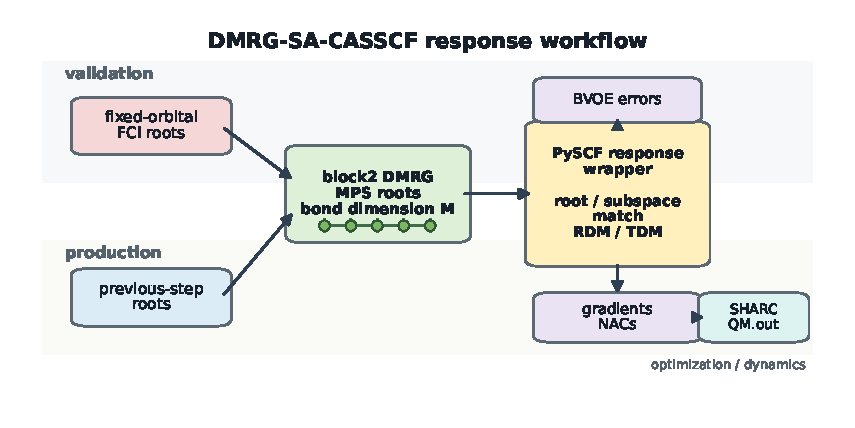
\includegraphics[width=0.92\textwidth]{figures/workflow_architecture.pdf}
\caption{General DMRG-SA-CASSCF response workflow.  The same solver layer
supplies target-state tracking, density matrices, transition density
matrices, and response operations to PySCF.  When FCI is available, it is used
only as a validation reference; production calculations use overlap-based
root following between successive geometries, macroiterations, or trajectory
steps.}
\label{fig:workflow}
\end{figure}

\section{Computational Details}

Calculations were performed with Python 3.11.14, PySCF 2.12.1, block2
0.5.3 through the pyblock2 Python interface, and SHARC 3.0.  The
SHARC-facing PySCF interface used in the trajectory smoke tests is included
with the code release.

All benchmark calculations used singlet state averaging over two roots with
equal weights.  The public systems are listed in Table~\ref{tab:systems}.
The bond-dimension response-error calculations used SA-CASSCF-converged
orbitals as the fixed orbital basis.  At those orbitals, the singlet
active-space Hamiltonian was rediagonalized with PySCF \texttt{direct\_spin0}
FCI for multiple roots, and the two lowest spin-adapted singlet roots defined
the reference CI vectors, energies, gradients, and derivative couplings.
Spin-adapted SU2 block2 DMRG
was then run at each selected bond dimension.  Isolated target states were
selected and phase-aligned by maximum overlap with the FCI reference.  When the
FCI root scan identified an exact or near-degenerate same-energy singlet
cluster, the DMRG candidate roots spanning that cluster were aligned to the
fixed FCI gauge by a subspace projection before derivative errors were
evaluated.  The same root-buffer assignment machinery used by the production
interface was enabled for dense or symmetry-related candidate subspaces.
Points shown in the convergence plots were required to have a minimum absolute
CI overlap of 0.98 with the assigned FCI roots and a converged corresponding
Lagrange-response solve.  All attempted bond dimensions are retained in the
machine-readable benchmark output.
Gradients are reported in m$\Eh$/Bohr and derivative couplings in atomic
units.

The FCI reference calculations used restricted Hartree--Fock orbitals
converged to $10^{-12}$, SA-CASSCF energy convergence of $10^{-12}$, and a
CASSCF gradient convergence threshold of $10^{-9}$.  The fixed-orbital FCI
polishing step used PySCF \texttt{direct\_spin0} with up to 20 roots
and an FCI convergence tolerance of $10^{-14}$; singlet roots were selected by
$\langle S^2\rangle$, same-energy clusters were identified with a
$10^{-4}$~$E_h$ threshold, and fixed-orbital residuals were recorded as QC
diagnostics.  The bond-dimension
scan used up to 100 DMRG sweeps, a DMRG
sweep tolerance of $10^{-14}$, and a Davidson threshold of $10^{-14}$ unless
noted otherwise.

The DMRG-SHARC trajectory smoke tests used NACDR coupling, two singlet
states, a 0.5 fs nuclear time step, and a 1.0 fs total propagation time.
The H$_2$ trajectory used SA(2)-DMRG-CASSCF(2,2)/STO-3G with $M=40$, eight
DMRG sweeps, and a DMRG sweep tolerance of $10^{-7}$.  The ethylene
trajectory used SA(2)-DMRG-CASSCF(2,2)/STO-3G with $M=60$, ten DMRG sweeps,
and a DMRG sweep tolerance of $10^{-8}$.  Both used CASSCF energy
convergence of $10^{-8}$ and CASSCF gradient convergence of $10^{-5}$.
These settings are intentionally small enough for public interface regression
tests and are not used to make mechanistic chemistry claims.

The large-active-space MPS-Krylov response benchmark used planar anthracene
with an AVAS-selected $\pi$ active space, CAS(14,14)/STO-3G, and the same
fixed-orbital reference protocol.  The validation FCI space contains
11,778,624 singlet determinants.  The runtime DMRG calculation selected
spin-adapted MPS roots without using FCI CI vectors; the cached FCI reference
was loaded only after the MPS response calculation to score the errors.  The
production row reported below used Boys-localized active orbitals\cite{Boys1960}
ordered by the principal molecular axis, $M=512$, response tolerance $10^{-8}$, MPS fit
tolerance $10^{-8}$, and 120 MPS-Krylov iterations for each response
right-hand side.  The gradient and derivative-coupling right-hand sides were
run as independent jobs and then combined for the final error analysis.

\begin{table}[h]
\centering
\scriptsize
\setlength{\tabcolsep}{3pt}
\caption{Public validation and benchmark systems.}
\label{tab:systems}
\begin{tabular}{P{0.18\textwidth}P{0.23\textwidth}P{0.18\textwidth}P{0.31\textwidth}}
\toprule
System & Basis sets & Active space & Role \\
\midrule
H$_4$ chain & STO-3G, 3-21G, 6-31G & CAS(4,4) & Small-system response validation \\
H$_2$O & STO-3G, 3-21G, 6-31G & CAS(4,4)/CAS(6,6) & Small polar molecule benchmark \\
N$_2$ & STO-3G, 3-21G, 6-31G & CAS(6,6) & Medium-active-space response validation \\
C$_2$ & STO-3G, 3-21G, 6-31G & CAS(8,8) & Larger active-space/root-tracking benchmark \\
Anthracene & STO-3G & CAS(14,14) & Large-active-space MPS-Krylov response benchmark \\
LiF & STO-3G, 3-21G, 6-31G & CAS(4,4) & Nonzero-NAC avoided-crossing benchmark \\
Ethylene & STO-3G, 3-21G, 6-31G & CAS(2,2) & SHARC-interface and $\pi/\pi^\ast$ benchmark \\
Butadiene & STO-3G, 3-21G, 6-31G & CAS(4,4) & Conjugated $\pi$-system benchmark \\
Formaldehyde & STO-3G, 3-21G, 6-31G & CAS(4,4) & Carbonyl excited-state benchmark \\
Benzene & STO-3G, 3-21G, 6-31G & CAS(6,6) & Aromatic $\pi$-space benchmark \\
\bottomrule
\end{tabular}
\end{table}

\section{Results and Discussion}
\label{sec:results}

\subsection{Validation Against FCI Active-Space References}

The implementation is covered by unit and integration tests for DMRG/FCI
energies, one- and transition-density matrices, MPS-to-FCI conversion,
analytic gradients, analytic derivative couplings, and SHARC output
formatting.  The current regression suite contains the public tests listed in
21 test files.  These tests verify both direct numerical agreement with FCI
active-space references in small active spaces and consistency between the
native MPS and PySCF-compatible solver paths.

\begin{table}[t]
\centering
\scriptsize
\caption{Validation layers included in the public test and benchmark suite.}
\label{tab:validation}
\begin{tabular}{p{0.25\textwidth}p{0.32\textwidth}p{0.34\textwidth}}
\toprule
Validation target & Public evidence & Quantity checked \\
\midrule
DMRG active-space solver
& Solver regression tests
& Energies, state density matrices, transition density matrices, and analytic
NAC pipeline consistency with FCI references. \\
MPS/FCI mapping
& Active-space map tests
& Round-trip mapping for CAS(2,2), CAS(4,4), and CAS(8,8) active spaces. \\
Response linear algebra
& Coupled-perturbed response tests
& Hermiticity, linearity, response-vector solves, and agreement between MPS
and FCI response operations in exactly recoverable cases. \\
MPS-Krylov response
& MPS-only response-vector tests
& Gradient and NAC RHS construction, MPS Krylov solves, MPS-only
initialization without dense CI roots, and MPS Lagrange nuclear assembly. \\
Fixed-orbital MPS-only SHARC path
& SHARC facade regression test
& Energies, dipoles, gradients, and NACs are evaluated from MPS roots with
only small \texttt{mc.ci} placeholders present at runtime. \\
Gradient and NAC derivatives
& Derivative regression tests
& Analytic gradients and derivative couplings against PySCF FCI active-space
references. \\
FCI-free runtime endpoint
& 27 public molecule/basis endpoint checks
& DMRG root selection and derivative evaluation run without FCI CI vectors;
FCI is loaded only afterward for error scoring. \\
SHARC interface
& H$_2$/ethylene trajectory smoke tests and MPS-Krylov SHARC-interface tests
& Repeated SHARC calls write \texttt{H}, \texttt{DM}, \texttt{GRAD},
\texttt{NACDR}, and \texttt{PHASES} blocks in \texttt{QM.out}; the
MPS-Krylov gradient/NAC path matches the projected-CI interface path in the
exact validation case. \\
\bottomrule
\end{tabular}
\end{table}

The FCI-free endpoint check was run for every molecule/basis entry in
Table~\ref{tab:systems}.  In all 27 cases, the DMRG endpoint selected roots and
evaluated gradients and derivative couplings without loading FCI CI vectors at
runtime; FCI data were loaded only after the endpoint calculation to score the
errors.  All gradient and derivative-coupling response solves converged.  The
largest post hoc FCI-scored gradient error was
$1.25\times10^{-6}$~m$\Eh$/Bohr for N$_2$/6-31G, and the largest derivative
coupling error was $3.79\times10^{-7}$~a.u. for LiF/6-31G.

The MPS-only response endpoint was additionally exercised on systems where
the active-space response vector is never represented as a dense CI array.
Hydrogen-chain calculations provide compact endpoint and timing checks, while
the anthracene CAS(14,14) calculation tests the same path in an active space
with an 11.8-million-determinant FCI validation target.  At $M=512$, the
strict MPS-Krylov response calculation gives maximum state-wise energy,
gradient, and derivative-coupling errors of $6.41\times 10^{-5}$ m$\Eh$,
$1.57\times 10^{-3}$ m$\Eh$/Bohr, and $9.11\times 10^{-6}$ a.u.,
respectively.  The strict response scan is monotonic over the completed
$M=64,128,256,512$ sequence: the maximum gradient error decreases from
$3.39$ to $0.368$, $0.0356$, and $1.57\times10^{-3}$ m$\Eh$/Bohr, while the
derivative-coupling error decreases from $2.22\times10^{-2}$ to
$2.52\times10^{-3}$, $1.68\times10^{-4}$, and $9.11\times10^{-6}$ a.u.

\begin{table}[t]
\centering
\scriptsize
\setlength{\tabcolsep}{3pt}
\caption{Fixed-orbital MPS-only response endpoint timings and large-active-space
accuracy.  No FCI reference or dense active-space response vector is used
during these runtime calculations; FCI data are used only for post hoc scoring
when a reference is available.}
\label{tab:mps-only-response}
\begin{tabular}{P{0.18\textwidth}P{0.13\textwidth}P{0.06\textwidth}P{0.12\textwidth}P{0.13\textwidth}P{0.25\textwidth}}
\toprule
System & Active space & $M$ & DMRG time (s) & Response wall time (s) & Post hoc validation \\
\midrule
H$_4$ chain/STO-3G & CAS(4,4) & 50 & 0.017 & 7.16 & exact-space endpoint \\
H$_{10}$ chain/STO-3G & CAS(10,10) & 200 & 3.81 & 751 & timing endpoint \\
Anthracene/STO-3G & CAS(14,14) & 512 & 848 & $3.67\times10^4$ &
$\Delta_g=1.57\times10^{-3}$ m$\Eh$/Bohr; $\Delta_d=9.11\times10^{-6}$ a.u. \\
\bottomrule
\end{tabular}
\end{table}

\begin{figure}[t]
\centering
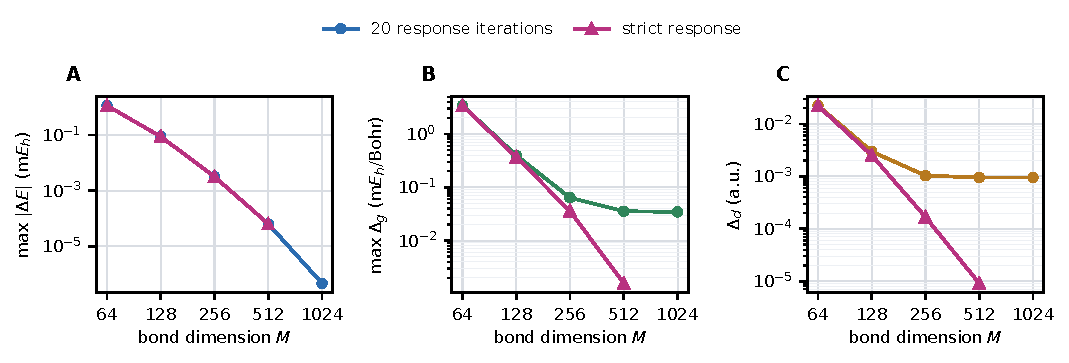
\includegraphics[width=\textwidth]{figures/anthracene_mps_krylov_response.pdf}
\caption{Anthracene CAS(14,14)/STO-3G fixed-orbital MPS-Krylov response
validation.  Circles show the standard 20-iteration response setting used to
scan bond dimension, and triangles show the strict response setting used for
production derivative validation.  Increasing $M$ converges the electronic
energies, while tightening the response solve reduces the gradient and
derivative-coupling errors to the FCI-scored strict-response values.}
\label{fig:anthracene-response}
\end{figure}

\subsection{FCI-Free Internal Consistency Validation Beyond the FCI Limit}
\label{sec:fcifree}

The validations above compare against an FCI active-space reference and are
therefore confined to active spaces where a determinant vector can be formed.
The derivative machinery here is designed to operate where that reference does
not exist, so its correctness must be established without one.  We use a
hierarchy of internal-consistency checks, each against the solver's own
SA-DMRG-CASSCF quantities rather than a higher-level reference: analytic
gradients against the central difference of the same SA-DMRG-CASSCF state
energy, $g^x_I \approx [E_I(\bfR+h\mathbf{e}_x)-E_I(\bfR-h\mathbf{e}_x)]/2h$, and
analytic derivative couplings against the bra-fixed finite difference of the
SA-DMRG-CASSCF wavefunction,
$d^x_{IJ}\approx[\langle\Psi_I(\bfR)|\Psi_J(\bfR+h\mathbf{e}_x)\rangle
-\langle\Psi_I(\bfR)|\Psi_J(\bfR-h\mathbf{e}_x)\rangle]/2h$.  The gradient check
needs only state energies and so is available at any active-space size; the
coupling check requires the cross-geometry wavefunction overlap, which we
evaluate in two ways.

For active spaces small enough to admit a determinant vector, the overlap is the
determinant-level L\"owdin formula over the active cross overlap.  Beyond that
size the overlap is formed MPS-natively: the displaced state is transported into
the reference DMRG driver and its active orbitals are rotated into the reference
basis (by the active cross overlap of the two geometries) before a same-basis
MPS overlap is taken, so no determinant expansion is constructed and the cost is
independent of the determinant-space dimension.  On HeH$^+$ CAS(2,2), where DMRG
is exact, the MPS-native derivative-coupling finite difference reproduces the
determinant-level finite difference to $1.6\times10^{-8}$ and the analytic
coupling to $1.3\times10^{-5}$, confirming that the FCI-free overlap route is
equivalent to the determinant route where both are available.

Table~\ref{tab:fcifree} collects the internal-consistency validation across the
active-space stair, together with the response certificate
(Eqs.~\eqref{eq:rho}--\eqref{eq:leak}) for each accepted solution.  At
CAS(20,20) the $3.41\times10^{10}$-determinant active space admits no FCI
vector; the gradient is validated by finite differences of the same DMRG energy
and the coupling route is the MPS-native overlap, with root continuity tracked
by the active-subspace singular values rather than an energy-sorted label.

\begin{table}[t]
\centering
\scriptsize
\setlength{\tabcolsep}{3pt}
\caption{Internal-consistency validation against the solver's own SA-DMRG-CASSCF
quantities, with the response certificate.  Entries marked \texttt{[pending]}
are filled from the completed large-active-space runs.  $\rho_z$ is the true
residual of the projected response equation, Eq.~\eqref{eq:rho}.}
\label{tab:fcifree}
\begin{tabular}{P{0.16\textwidth}P{0.10\textwidth}P{0.10\textwidth}P{0.06\textwidth}P{0.18\textwidth}P{0.14\textwidth}P{0.10\textwidth}}
\toprule
System & Active space & Det.\ dim. & FCI? & Internal check & Abs.\ error & $\rho_z$ \\
\midrule
HeH$^+$ & CAS(2,2) & $4$ & yes & MPS-native NAC FD vs det.\ FD & $1.6\times10^{-8}$ & \texttt{[pending]} \\
polyene & CAS(10,10) & $6.4\times10^{4}$ & yes & MPS-native NAC FD vs det.\ FD & \texttt{[pending]} & \texttt{[pending]} \\
polyene & CAS(14,14) & $1.2\times10^{7}$ & yes & gradient FD of DMRG energy & \texttt{[pending]} & \texttt{[pending]} \\
polyene & CAS(20,20) & $3.41\times10^{10}$ & \textbf{no} & gradient FD of DMRG energy & \texttt{[pending]} & \texttt{[pending]} \\
\bottomrule
\end{tabular}
\end{table}

\subsection{Finite-Bond-Dimension Response Error}

Figure~\ref{fig:bvoe} shows representative fixed-orbital
bond-dimension response-error curves for points that pass the root-overlap and
response-equation convergence checks described above.  The selected systems
cover small active spaces, CAS(6,6) and CAS(8,8) examples, nonzero derivative
couplings, and a public SHARC-interface molecule.  These curves show
reduction of the derivative error as $M$ is increased and recover the FCI
active-space limit at high $M$.  The high-$M$ gradient errors in
Table~\ref{tab:largestm} are reported in m$\Eh$/Bohr; values near
$10^{-4}$ in this column correspond to $10^{-7}$ $\Eh$/Bohr and are well
below the $0.1$ m$\Eh$/Bohr reference line in Figure~\ref{fig:bvoe}.  The NAC
column is an absolute vector error and is interpreted together with the
benchmark matrix in Figure~\ref{fig:highm}.  The full scan, including low-$M$
points excluded from accuracy claims by the overlap or Lagrange-response QC
criteria, is provided with the benchmark data.  In the N$_2$ scans, the
homonuclear geometry gives a symmetry-suppressed derivative coupling and a
root-labeling problem for low-rank truncated CI spaces: several low- and
intermediate-$M$ DMRG roots are accurate enough energetically to be nearby
states but do not satisfy the root-overlap criterion for a root-by-root FCI
derivative comparison.  The high-$M$ points recover unit overlap with the FCI
reference, sub-$10^{-6}$ $\Eh$/Bohr gradient errors, and NAC errors near
$10^{-8}$ a.u.

\begin{table}[t]
\centering
\scriptsize
\setlength{\tabcolsep}{3pt}
\caption{Representative largest-$M$ fixed-orbital response errors from the
public benchmark scan.  The full molecule/basis matrix is summarized in
Figure~\ref{fig:highm}.}
\label{tab:largestm}
\begin{tabular}{P{0.18\textwidth}P{0.12\textwidth}P{0.06\textwidth}P{0.15\textwidth}P{0.12\textwidth}P{0.23\textwidth}}
\toprule
System & Active space & $M$ & $\Delta_g$ (m$\Eh$/Bohr) & $\Delta_d$ & Role \\
\midrule
H$_4$/STO-3G & CAS(4,4) & 200 & $1.06\times10^{-12}$ & $2.98\times10^{-15}$ & High-$M$ exact-rank check \\
H$_2$O/6-31G & CAS(6,6) & 200 & $3.35\times10^{-8}$ & $1.45\times10^{-9}$ & Polar molecule benchmark \\
N$_2$/6-31G & CAS(6,6) & 200 & $1.19\times10^{-6}$ & $9.19\times10^{-9}$ & Medium CAS benchmark \\
C$_2$/6-31G & CAS(8,8) & 800 & $4.75\times10^{-7}$ & $1.06\times10^{-8}$ & Larger active-space benchmark \\
LiF/6-31G & CAS(4,4) & 200 & $1.35\times10^{-12}$ & $5.84\times10^{-7}$ & Avoided-crossing benchmark \\
Ethylene/6-31G & CAS(2,2) & 200 & $5.98\times10^{-11}$ & $1.22\times10^{-13}$ & SHARC-interface benchmark \\
Butadiene/6-31G & CAS(4,4) & 200 & $1.10\times10^{-9}$ & $2.22\times10^{-10}$ & Conjugated $\pi$ benchmark \\
Formaldehyde/6-31G & CAS(4,4) & 200 & $2.73\times10^{-11}$ & $5.97\times10^{-14}$ & Carbonyl benchmark \\
Benzene/6-31G & CAS(6,6) & 200 & $5.88\times10^{-7}$ & $2.45\times10^{-8}$ & Aromatic $\pi$ benchmark \\

\bottomrule
\end{tabular}
\end{table}

\begin{figure}[tbp]
\centering
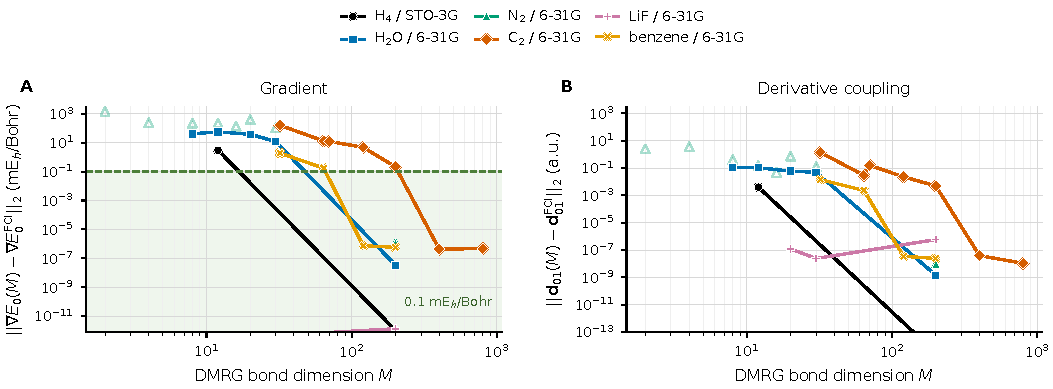
\includegraphics[width=\textwidth]{figures/bvoe_phase2.pdf}
\caption{Fixed-orbital bond-dimension response-error convergence for public
benchmark systems.  Gradient errors are reported in m$\Eh$/Bohr and
nonadiabatic coupling errors in atomic units.  Filled symbols connected by
lines pass the uniform benchmark QC: minimum assigned root overlap with the
FCI reference of at least 0.98 and converged gradient and NAC response
equations.  Pale open triangles mark computed N$_2$/6-31G points that fail
one of these QC filters and are not used for convergence claims.  Points use
the same fixed spin-adapted FCI reference protocol; near-degenerate reference
clusters are compared after the uniform subspace-alignment step described in
the text.}
\label{fig:bvoe}
\end{figure}

\begin{figure}[tbp]
\centering

\includegraphics[width=0.96\textwidth]{figures/bvoe_highm_heatmap.pdf}
\caption{Largest-$M$ derivative errors across the public molecule/basis
matrix.  Color encodes the base-10 logarithm of the error, while each cell
reports the corresponding gradient error in m$\Eh$/Bohr or NAC error in
atomic units.}
\label{fig:highm}
\end{figure}

\clearpage

\subsection{SHARC Interface-Contract Regression Tests}

The public H$_2$ and ethylene tests request the Hamiltonian, dipole matrices,
gradients for both singlet states, and derivative couplings in SHARC NACDR
mode.  Each run completed three SHARC frames, corresponding to steps
0, 1, and 2, and the final \texttt{QM.out} file contained all data blocks
requested by SHARC.  These tests confirm that the DMRG-backed PySCF object
satisfies the repeated-call data contract expected by SHARC for energies,
dipoles, gradients, derivative couplings, and phase bookkeeping.  They verify
the interface contract only: they are not claimed as a validation of
large-active-space nonadiabatic dynamics, for which the per-call response cost
(Section~\ref{sec:results}) is the governing constraint.  The repeated-call
robustness of the same backend over a longer torsional scan is examined
separately in Section~\ref{sec:repeated-call}.

\begin{table}[t]
\centering
\scriptsize
\setlength{\tabcolsep}{3pt}
\caption{SHARC interface-contract regression tests (data-block delivery over
repeated calls; not a dynamics validation).}
\label{tab:sharc-smoke}
\begin{tabular}{P{0.14\textwidth}P{0.28\textwidth}P{0.08\textwidth}P{0.15\textwidth}P{0.25\textwidth}}
\toprule
System & Electronic-structure model & $M$ & Trajectory frames & Final \texttt{QM.out} blocks \\
\midrule
H$_2$ & SA(2)-DMRG-CASSCF(2,2)/STO-3G & 40 & 3 (steps 0--2) & \texttt{H}, \texttt{DM}, \texttt{GRAD}, \texttt{NACDR}, \texttt{PHASES} \\
Ethylene & SA(2)-DMRG-CASSCF(2,2)/STO-3G & 60 & 3 (steps 0--2) & \texttt{H}, \texttt{DM}, \texttt{GRAD}, \texttt{NACDR}, \texttt{PHASES} \\
\bottomrule
\end{tabular}
\end{table}

\subsection{Root and Subspace Tracking Near a Degeneracy}
\label{sec:tracking}

Where electronic states approach degeneracy an energy-sorted root label is not a
reliable identity, so the implementation follows roots by the cross-geometry
overlap of the active-space wavefunctions rather than by energy order.  To show
that this remains stable through an avoided crossing we scan the LiF
ionic/covalent crossing of the two lowest singlets at CAS(6,6) and report, as a
function of the bond length, the two state energies and their gap, the
cross-geometry overlap matrix between successive geometries, and the smallest
singular value of the active-subspace cross overlap; the analytic derivative
coupling and its finite-difference reference are overlaid across the crossing
in a single multi-panel figure.  The singular values remain near unity away from
the crossing and degrade smoothly through it, so the subspace is tracked
continuously even where individual root labels would interchange.
% Figure assembled from the LiF CAS(6,6) bond-length scan (data run in progress).

\subsection{Repeated-Call Robustness}
\label{sec:repeated-call}

Nonadiabatic dynamics calls the electronic-structure backend once per nuclear
step, so the relevant test is the stability and cost of repeated derivative
evaluations along a path rather than a single point.  We walk ethylene through
the C=C torsion (the classic S$_0$/S$_1$ approach) at CAS(2,2) and, at each step,
solve the two state gradients and their derivative coupling, once from a zero
guess and once with same-geometry recycling, recording the response wall time and
iteration count for both, the certified true residual, the state energies and
gap, and the root continuity to the previous step.  At a fixed geometry the
response operator is identical for the gradients and the coupling, so a recycled
warm start from a prior solve reuses its Arnoldi subspace; the second state
gradient then converges in a small number of iterations while the accepted
solution is invariant to the warm start.
% Per-step timings/iterations/continuity assembled from the ethylene torsion
% scan (data run in progress).

\section{Conclusions}

We have implemented analytic SA-DMRG-CASSCF gradients and nonadiabatic
couplings in a PySCF/pyblock2 workflow with a certified, FCI-free response
path and exposed the backend through a SHARC-compatible interface.  Where an
FCI reference exists, the derivatives are validated against it; where it does
not, they are validated against finite differences of the solver's own
SA-DMRG-CASSCF energies and, for derivative couplings, against an MPS-native
cross-geometry overlap of the SA-DMRG-CASSCF wavefunction that forms no
determinant expansion.  Every accepted response solution is gated by the true
residual of the projected coupled-perturbed equation and reports its
root-projector leakage, so convergence is asserted without reference to an
external benchmark.  The active-space response is never stored as a dense
determinant array, which lets the derivative machinery reach active spaces,
up to CAS(20,20), where an FCI vector cannot be formed.  The present work
establishes certified FCI-free derivative evaluation and SHARC-compatible data
delivery for singlet, closed-shell active spaces; long-time large-active-space
DMRG-SHARC dynamics remains cost-sensitive and is not claimed here.  Extending
the certified response to open-shell and spin-orbit-coupled manifolds, and
reducing the per-call response cost, are the natural next steps.

\section*{Supporting Information}

Supporting Information: benchmark inputs, full convergence tables,
regression-test summary, and SHARC DMRG-CASSCF trajectory smoke-test files.

\section*{Data and Code Availability}

The public code bundle contains the response implementation, tests, benchmark
drivers, benchmark summaries, plotting scripts, and the ethylene SHARC
interface regression and trajectory smoke-test examples.  The repository is:
{\small\url{https://github.com/yurika1030sakura/mps-casscf-gradient-nac-sharc}.}
All input files, generated benchmark summaries, and plotting scripts needed to
reproduce the public figures and tables are included in the repository.

\section*{Acknowledgments}

Y.L. thanks Prof. Christina M. Woo for mentorship and for providing a
supportive research environment in which this methodological project was
carried out.  Y.L. thanks Prof. Richard Liu for helpful discussions.
Computations were performed on the Harvard FAS Research Computing Cannon
cluster.  No specific external grant funding was used for this work.

\bibliography{references}

\end{document}
